\chapter{Metodologías a usar en el proyecto}
\label{ch:metodologias}
En este capítulo se explicaran las diferentes metodologías que serán utilizadas para desarrollar el proyecto, estas incluyen metodologías de desarrollo ágil, diseño centrado en el usuario y el proceso de desarrollo de videojuegos.

\section{Metodologías de desarrollo ágil}
El desarrollo del proyecto se llevará a cabo utilizando metodologías de desarrollo ágil, estas surgen a partir del Manifiesto Ágil \cite{beck}, más concretamente se utilizarán elementos de Scrum, que se basa en un desarrollo iterativo, en el que el producto se irá construyendo por etapas, y será testeado en cada una de dichas etapas, permitiendo así una temprana solución de errores, y añadiendo también un valor extra al producto al haber sido testeado varias veces durante el desarrollo por usuarios reales. El desarrollo ágil también permitirá una mas sencilla organización del proyecto, en la que a partir de un plan de entregas inicial se van organizando las iteraciones para ir cumpliendo los objetivos de estas entregas.\\

\newpage

En la Figura \ref{figura-agile} se puede observar un esquema del desarrollo por iteraciones:

\begin{figure}[h]
  \centering
  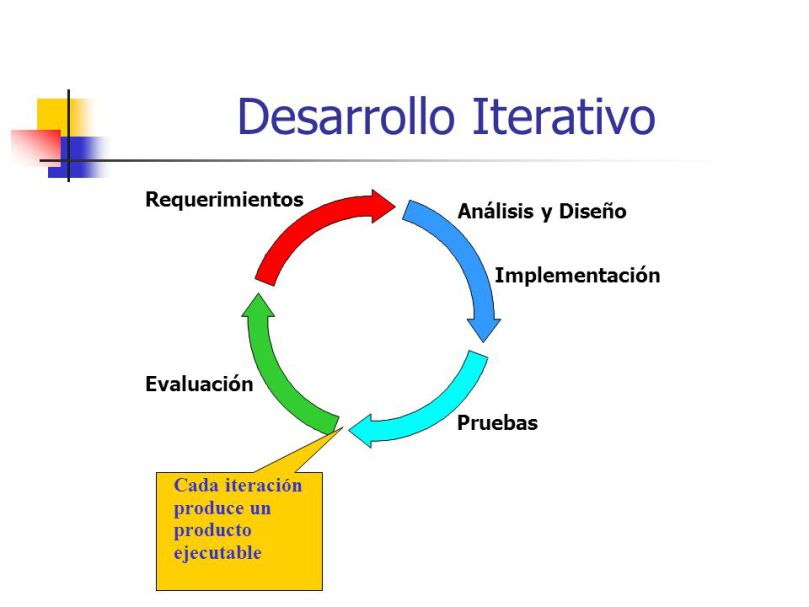
\includegraphics[scale=0.45]{agile}
  \caption{Imagen que muestra un proceso de desarrollo iterativo.\protect\footnotemark}
  \label{figura-agile}
\end{figure}

\footnotetext{Yuukiter, {\em Desarrollo de Software Iterativo}, RUP, Recuperado de \\
\url{https://rupnoobs.wordpress.com/2016/03/10/desarrollo-de-software-iterativo/}, (11 de marzo de 2016).}

El primer elemento relevante que se utilizará en el desarrollo son las historias de usuario, que nos permitirán establecer unos requisitos iniciales para la aplicación de una forma sencilla y completa. A estas historias de usuario se les asignará una entrega para la que la historia deberá estar completa y una iteración en la que se lleva a cabo, de forma que se obtiene de una forma organizada cuales son las partes del producto que tienen que estar listas para cada entrega.\\

Dentro de cada entrega puede existir una o varias iteraciones, estas se planificarán al inicio cuando se define dicha iteración, y contendrá las tareas a realizar en cada iteración, que suelen ser historias de usuario, pero que también pueden incluir otras tareas de documentación o tareas necesarias para el desarrollo, que no necesariamente son una historia de usuario, como por ejemplo, obtener los modelos 3D que serán necesarios para el juego.\\

Por otro lado se realizarán entregas, que quedán detalladas en el plan de entregas creado al inicio del proyecto. Al final de cada entrega se obtendrá un producto, que será testeado tanto por el desarrollador como por los usuarios.

\subsection{Diseño centrado en el usuario}
Uno de los principios del desarrollo ágil es la satisfacción del usuario, por tanto, el desarrollo de este proyecto también esta enfocado en el diseño centrado en el usuario \cite{sanchez}, de forma que, gracias a una organización por iteraciones y con entregas, se obtenga una retroalimentación por parte del usuario en cada entrega.\\

El proceso por iteraciones del diseño centrado en el usuario que se puede observar en la Figura \ref{figura-iteraciones}, se integra con las entregas iniciales que es cuando se esta llevando a cabo el diseño, y por tanto, donde quedará definido este, las etapas de una iteración para el diseño centrado en el usario son diferentes a las de una iteración del desarrollo, ya que estas especificamente se centran en el diseño.

\begin{figure}[h]
  \centering
  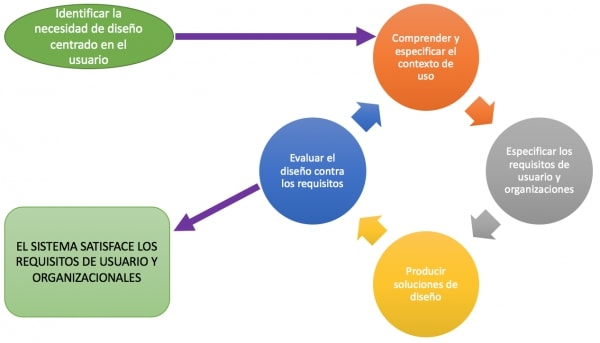
\includegraphics[scale=0.6]{iteraciones}
  \caption{Imagen que muestra un proceso de desarrollo iterativo centrado en el usuario.\protect\footnotemark}
  \label{figura-iteraciones}
\end{figure}

\footnotetext{Alfredo, {\em ¡Diseña centrándote en el usuario!}, Time of Software, Recuperado de \\
\url{http://timeofsoftware.com/disena-centrandote-en-el-usuario/}, (16 de enero de 2017).}

\newpage

Estas etapas son:
\begin{itemize}
  \item Se especifica el contexto de uso para entender la situación del usuario.
  \item Basado en dicho contexto se establecen los requisitos.
  \item Una vez obtenidos los requisitos se hacen las soluciones de diseño.
  \item Finalmente se evalua el producto probandolo con el usuario.
\end{itemize}

Las evaluaciones del diseño al final de cada iteración coinciden con las entregas iniciales, que suponen una fecha en la que se presenta un producto al usuario, y se realizan pruebas sobre dicho producto, de forma que el usuario esta utilizando el producto, lo que permite una realimentación por parte del usuario de forma periodica, para detectar fallos o posibles mejoras sobre el diseño a tiempo, y solventarlos, de manera que el producto final, sea lo mas sencillo de utilizar por el usuario, este proceso a su vez, esta incrementando el valor del producto, preparandolo para que en el momento que se lance al mercado, los fallos sean mínimos y la experiencia del usuario final sea excelente.\\

Por tanto, este proceso es beneficioso para el usuario, ya que todo el desarrollo esta centrado en que el producto le ofrezca una buena experiencia, ya que al fin y al cabo, es el usuario el que estrá en contacto con el producto a diario. Y todo esto es posible ya que todo el proceso de desarrollo está orientado al usuario y su experiencia utilizando el producto.

\section{Desarrollo de videojuegos}
